\documentclass[a4paper]{article}
\pdfoutput=1
\usepackage[utf8]{inputenc}
\usepackage{jheppub}
\usepackage{overpic}
\usepackage{subcaption}
\usepackage{fancybox}
\usepackage{float}
\usepackage{amsfonts}
\usepackage{amsmath}
\usepackage{amsbsy}
\usepackage{graphicx}
\usepackage{amssymb}
\usepackage{amsthm}
\usepackage{bm}
\usepackage{comment}
\usepackage{epsfig}
\usepackage{latexsym}
\usepackage{pdflscape}
\usepackage{color}
\usepackage{slashed}
\usepackage{tikz}
\usetikzlibrary{arrows.meta,decorations.markings}

\tikzset{
  mid arrow/.style={
    postaction={
      decorate,
      decoration={
        markings,
        mark=at position 0.5 with {\arrow{Stealth[length=6pt,width=6pt]}}
      }
    }
  }
}

\usepackage{cancel}
\usepackage{xcolor}
\usepackage{braket}
\usepackage{empheq}
\usepackage{graphicx} % Allows including images
\usepackage{tikz-3dplot}
% réglage de la vue 3D : élévation=20°, azimut=110°
\tdplotsetmaincoords{20}{110}
\usetikzlibrary{decorations.pathreplacing,calc}
\usetikzlibrary{decorations.pathmorphing}

\definecolor{blue5}{rgb}{0, 0, 0.66666}
\definecolor{red4}{rgb}{0.8, 0, 0}
\definecolor{navyblue}{rgb}{0, 0.2745, 0.67843}
\definecolor{cornflowerblue}{rgb}{0.388235, 0.6941176, 0.898039}
\definecolor{forestgreen}{rgb}{0.13, 0.55, 0.13}
\usetikzlibrary{decorations.text,decorations.pathmorphing}

%Removes Header------------------------------------
\makeatletter
\def\@fpheader{\relax}
\makeatother



\usepackage{orcidlink}

%\DeclareMathOperator{\tr}{tr}
\DeclareMathOperator{\pf}{pf}
\DeclareMathOperator{\Ai}{Ai}
\DeclareMathOperator{\vol}{vol}
\DeclareMathOperator{\sgn}{sgn}
\DeclareMathOperator{\sn}{sn}
\DeclareMathOperator{\cn}{cn}
\DeclareMathOperator{\dn}{dn}
\DeclareMathOperator{\cd}{cd}
\DeclareMathOperator{\Det}{Det}
\DeclareMathOperator{\sech}{sech}
% \DeclareMathOperator{\tr}{tr}

\newcommand{\beq}{\begin{eqnarray}}
\newcommand{\eeq}{\end{eqnarray}}
\newcommand{\bea}{\begin{eqnarray}}
\newcommand{\eea}{\end{eqnarray}}
\newcommand{\be}{\begin{equation}}
\newcommand{\ee}{\end{equation}}
\newcommand{\bq}{\begin{equation}}
\newcommand{\eq}{\end{equation}}
\newcommand{\unit}{1\!\!1}
\newcommand{\half}{\frac{1}{2}}
\newcommand{\nn}{\nonumber}
\newcommand{\no}{\nonumber}
\def\tb{\tilde{\beta}}
\newcommand{\mpl}{M_{\rm Pl}}
\def\k{\kappa}

\newcommand{\bto}{\bar{\tau}^{\textbf{I}}}
\newcommand{\btt}{\bar{\tau}^{\textbf{II}}}




%%% Other definitions


\def\sp{\;\;\;,\;\;\;}
\def\l{\lambda}
%\def\z{\zeta}
\def\lab{\label}
\def\f{H}
\def\La{\Lambda}
\def\z{\zeta}
\def\t{\tau}
\def\e{\epsilon}
\def\o{\omega}
\def\le{\left}
\def\ri{\right}
\def\y{\psi}
\def\half{\frac12}
\def\q{\theta}
\def\cO{{\cal O}}
\def\m{\mu}
\def\n{\nu}
\def\td{\tilde}
\def\d{\delta}
\def\6{\partial}
\def\de{\partial}
\def\del{\nabla}
\def\ls{\ell_s}
\def\a{\alpha}
\def\b{\beta}
\def\lab{\label}
\def\parl{\parallel}
\def\tom{\tilde{\o}}
\def\dA{\dot{A}}
\def\dh{\dot{h}}
\def\df{\dot{f}}
\def\dX{\dot{X}}
\def\bo{\bar{\o}}
\def\r{x}
\def\bo{b_0}
\def\br{\bar{r}}
\def\dx{\delta X^\parl}
\def\dxy{\delta X^2}
\def\dxz{\delta X^3}
\def\ol{\overline}
\def\GM#1{\textit{[GM: #1]}}
\def\g{\gamma}
\def\s{\sigma}
\def\tr{{\rm Tr}}
\def\eps{\epsilon}
\def\fb{f}
\def\rd{\rm d}
\newcommand{\bom}[1]{\fboxsep2mm\fbox{
           $ \displaystyle{ #1} $}}
           
           \newcommand{\rar}{\rightarrow}
\newcommand{\bb}{\mathbb}
\newcommand{\mc}{\mathcal}
\newcommand{\im}{\mathrm{Im}}
\newcommand{\re}{\mathrm{Re}}
\newcommand{\mi}{\sqrt{|\mathcal{I}_4|}}


\def\lab{\label}
\def\le{\left}
\def\ri{\right}
\def\6{\partial}
\def\eps{\epsilon}


% Color definitions
\newcommand{\red}[1]{{\color{red} #1 \color{black}}}
\newcommand{\blue}[1]{{\color{blue} #1 \color{black}}}
\newcommand{\green}[1]{{\color{green} #1 \color{black}}}
\newcommand{\yellow}[1]{{\color{yellow} #1 \color{black}}}
\newcommand{\purple}[1]{{\color{purple} #1 \color{black}}}


% Comment Abbreviations
\newcommand{\IT}[1]{{\red{IG: #1}}} %Ioannis
\newcommand{\PB}[1]{{\blue{PB: #1}}} % Panos
\newcommand{\OP}[1]{{\green{OP: #1}}} % Olga
\newcommand{\PG}[1]{{\purple{PG: #1}}} % Paul

\title{Notes on Axionic wormholes}

\author[a]{Panos Betzios\orcidlink{0000-0002-5350-9404},}
\author[b]{Paul Ghiringhelli,}
\author[b]{Olga Papadoulaki\orcidlink{0000-0001-5302-2930}}
\affiliation[a]{\href{https://www.ugent.be/we/physics-astronomy/en}{Department of Physics and Astronomy},
Ghent University, \\ Krijgslaan, 281-S9, 9000 Gent, Belgium}
\affiliation[b]{\href{https://www.cpht.polytechnique.fr/?q=en}{CPHT, CNRS, École polytechnique, Institut Polytechnique de Paris},  91120 Palaiseau, France}

\emailAdd{panos.betzios@ugent.be}
\emailAdd{paul.ghiringhelli@polytechnique.edu}
\emailAdd{olga.papadoulaki@polytechnique.edu}





\abstract{...}

\keywords{...}


\begin{document}
\maketitle
\flushbottom


%%%%%%%%%%%%%%%%%%%%%%%%%%%%%%%%%%%%%%%%%%%%%%%%%%%%%%%%%%

\section{Action principle and equations of motion}
Our starting point is the following action
\begin{equation}\label{eq:startingaction}
\mathcal{S} = \int d^Dx \sqrt{g}\left[\frac{1}{2\kappa}\left(-\mathcal{R}+2\Lambda\right) +\frac{1}{2(D-1)!}H_{\mu... \nu}H^{\mu...\nu}\right]\,.
\end{equation}
H is a $(D-1)$-form field strength satisfying the Bianchi identity $dH=0$. Thus, one can always write locally $H=dB$ where $B$ is a $(D-2)$-form field. The equations of motion are simply $d \star H =0$. We can see classically that the dynamics of $H$ is locally governed by a pseudo-scalar field $\chi$ defined as $\star H= i\,d \chi$.

That holds at the quantum level. To see this we introduce $\chi$ as a Lagrangian multiplier in the following 1st class formalism action

\begin{equation}
  \begin{aligned}
    \mathcal{S}_{1st} &= \int d^Dx \frac{\sqrt{g}}{2\kappa}\left(-\mathcal{R}+2\Lambda\right) +\frac{1}{2}\int H \wedge \star H +  \int\chi \wedge dH\\
    &= \int d^Dx \frac{\sqrt{g}}{2\kappa}\left(-\mathcal{R}+2\Lambda\right) +\frac{1}{2}\int H \wedge \star H -  \int d\chi \wedge H + \mathcal{S}_{\partial M}\,.
  \end{aligned}
\end{equation}
where
\begin{equation}
  \mathcal{S}_{\partial M}= \int_{\partial M}\chi \wedge H\,.
\end{equation}
The path-integral whose action is defined by~\eqref{eq:startingaction} can be recovered by integrating out $\chi$ imposing Bianchi's identity. In the meantime, the action is quadratic in $H$ so we can integrate out $H$ as well by solving its equation of motion
\begin{equation}
  H =  \star \,d \chi \Rightarrow \star H = (-1)^{D-1} d \chi\,.
\end{equation}
Indeed, inserting back into the action we get
\begin{equation}
\mathcal{S}_{\chi} = \int d^Dx \frac{\sqrt{g}}{2\kappa}\left(-\mathcal{R}+2\Lambda\right) - \frac{1}{2} \int d \chi \wedge \star d\chi - \int_{\partial M} \chi \wedge \star d\chi\,.
\end{equation}
Instanton configurations have the effect of modifying the action by mean of a non-perturbative potential $V_{\rm np}(\chi)$ so that the total action in the pseudo-scalar variable reads
\begin{equation}\label{eq:liftnonperturbative}
  \mathcal{S}=\int d^Dx \sqrt{g}\left[\frac{1}{2\kappa}\left(-\mathcal{R}+2\Lambda\right)-\frac{1}{2}\partial_\mu\chi \partial^\mu \chi + V_{\rm np}(\chi)\right]+ \mathcal{S}_{GHY} + S_{\partial M}\,.
\end{equation}
We emphasize that this will not be the case for running solutions. The charge is a running parameter

We look for homogeneous and isotropic solutions of the form
\begin{equation}
  ds^2= N^2(\tau)d\tau^2 + a^2(\tau) d \Sigma_{d}^2\sp \chi=\chi(\tau)\,.
\end{equation}
We obtain the following expressions for the determinant of the metric and the Ricci scalar
\begin{equation}
  \sqrt{g}=N a^d\sp \mathcal{R}=-\frac{2d}{N} \frac{d}{d\tau}\left(\frac{a'}{aN}\right)+d(d-1)\frac{k}{a^2}-d(d+1)\left(\frac{a'}{aN}\right)^2\,.
\end{equation}
Finally, let's also mention the form of the Gibbons-Hawking term
\begin{equation}\label{eq:GHY}
  \begin{aligned}
    \mathcal{S}_{GHY} = -\frac{1}{\kappa}\int_{\partial M} d^d x \sqrt{h} K = -\frac{1}{\kappa}\frac{\partial_\tau}{N}V_d (a^d) = -\frac{d V_d a' a^{d-1}}{\kappa N}\,. 
  \end{aligned}
\end{equation}
Hence the Lagrangian density of the Einstein-Hilbert part of the action reads
\begin{equation}
  \begin{aligned}
    \mathcal{L}_{EH} &= -\frac{N a^d}{2\kappa}\left[-\frac{2d}{N} \frac{d}{d\tau}\left(\frac{a'}{aN}\right)+d(d-1)\frac{k}{a^2}-d(d+1)\left(\frac{a'}{aN}\right)^2+2\Lambda\right]\\
    &= -\frac{1}{2\kappa}\left[\frac{d(d-1)(a')^2 a^{d-2}}{N} + d(d-1) N k a^{d-2} - 2 N \Lambda a^{d}\right] + \frac{d}{d\tau}\left[\frac{d a^{d-1} a' }{\kappa N}\right]\,.
  \end{aligned}
\end{equation}
The boundary term coming from this total derivative will get exactly canceled by the Gibbons-Hawking term (see ~\eqref{eq:GHY}).
We also have
\begin{equation}
  \mathcal{L}_{\chi}=-\frac{a^d}{2N}(\partial_\tau \chi)^2 + N a^{d} V_{\rm np}(\chi)\,.
\end{equation}
Also, note that taking the trace of Einstein equation allows one to evaluate the on-shell action as a function of the on-shell solution $\chi$. Indeed,
\begin{equation}
\begin{aligned}
  G &= \kappa T^{\chi} - \Lambda D \Rightarrow \mathcal{R}\left(1-\frac{D}{2}\right)=\kappa T^{\chi} - \Lambda D\,,\\
  T_{\mu \nu}^{\chi}&= -\partial_\mu \chi \partial_\nu \chi -g_{\mu\nu}\left(-\frac{1}{2}(\partial_\lambda \chi)^2+V_{\rm np}(\chi)\right) \Rightarrow T^{\chi}=\left(\frac{D}{2}-1\right)(\partial_\lambda \chi)^2 - D V_{\rm np}(\chi)\,.
\end{aligned}
\end{equation}
After some manimpulations one obtains
\begin{equation}
  \frac{-\mathcal{R}+2\Lambda}{2\kappa}=\frac{1}{2}(\partial_\lambda \chi)^2-\frac{DV_{\rm np}}{D-2}-\frac{2\Lambda}{\kappa(D-2)}\,.
\end{equation}
We also have the additional boundary terms
\begin{equation}
  \begin{aligned}
    \mathcal{S}_{GHY} = -\frac{dV_{d}a'a^{d-1}}{\kappa N}\Bigg|_{\partial M}\sp \mathcal{S}_{\partial M} = -\frac{V_d}{N}\,a^d \chi \partial_\tau \chi \Bigg|_{\partial M}\,.
  \end{aligned}
\end{equation}
The on-shell action thus takes the simple expression
\begin{equation}\label{eq:on-shell_action}
  S^{\rm on-shell} = V_{d}\,\int d\tau N a^{d}\left(-\frac{2V_{\rm np}}{D-2}-\frac{2\Lambda}{\kappa(D-2)}\right)+\mathcal{S}_{GHY}+\mathcal{S}_{\partial M}\,.
\end{equation}
This on-shell action is an important quantity since the final question one should answer is how it evolves as a function of the number of bubbles. The flow paramater is $u= N \tau$. Remark that the on-shell action does not depend on the kinitic term and can be easily deduced from this formula once $\chi$ and the scale factor is known. 

Let's now derive the equation of motions. The simplest one is obtain by varying wrt to $\chi$ yielding
\begin{equation}
  \partial_\tau\left(\frac{a^d}{N}\partial_\tau \chi\right)+Na^{d}\partial_{\chi}V_{np}(\chi)=0\,.
\end{equation}
Varying with respect to $a$ in $\mathcal{L}_{EH}+\mathcal{L}_{\chi}$ yields
\begin{equation}
  \begin{aligned}
    &\Bigg[-\frac{d a^{d-1}}{2N}(\partial_\tau \chi)^2+d N a^{d-1} V_{\rm np}(\chi)-\frac{1}{2\kappa}\Big(\frac{d(d-1)(d-2)}{N}a'^2a^{d-3}\\
    &+d(d-1)(d-2)kNa^{d-3}-2N \Lambda d a^{d-1} \Big)\Bigg]\delta a
    -\frac{1}{2\kappa}\frac{d(d-1)2a'a^{d-2}}{N}\delta(a')\,.
  \end{aligned}
\end{equation}
Thus, integrating by parts the second term
\begin{equation}
  \begin{aligned}
    &\Bigg[-\frac{d a^{d-1}}{2N}(\partial_\tau \chi)^2+d N a^{d-1} V_{\rm np}(\chi)-\frac{1}{2\kappa}\Bigg(\frac{d(d-1)(d-2)}{N}a'^2a^{d-3}\\
    &+d(d-1)(d-2)kNa^{d-3}-2N \Lambda d a^{d-1} -2d(d-1)\frac{d}{d\tau}\Bigg(\frac{a' a^{d-2}}{N}\Bigg)\Bigg)\Bigg]\delta a\,.
  \end{aligned}
\end{equation}
We thus get the following equation of motion
\begin{equation}
  \begin{aligned}
    &\frac{d a^{d-1}}{2N}(\partial_\tau \chi)^2-d N a^{d-1} V_{\rm np}(\chi)+\frac{1}{2\kappa}\Bigg(\frac{d(d-1)(d-2)}{N}a'^2a^{d-3}\\
    &+d(d-1)(d-2)kNa^{d-3}-2N \Lambda d a^{d-1} -2d(d-1)\frac{d}{d\tau}\Bigg(\frac{a' a^{d-2}}{N}\Bigg)\Bigg)=0\,.
  \end{aligned}
\end{equation}
Finally, varying wrt to N we generate a third (non-independent) equations
\begin{equation}
  \begin{aligned}
    a^d V_{\rm np}(\chi)+\frac{a^d}{2N^2}(\partial_\tau \chi)^2-\frac{1}{2\kappa}\left[d(d-1)ka^{d-2}-2\Lambda a^d -\frac{d(d-1)a'^2 a^{d-2}}{N^2}\right]=0\,.
  \end{aligned}
\end{equation}
Let's summurize the set of equations here for general ($k,\,\Lambda,\,N$)
\begin{equation}
  \begin{aligned}
    \partial_\tau\left(\frac{a^d}{N}\partial_\tau \chi\right)+Na^{d}\partial_{\chi}V_{np}(\chi)&=0\,.\\
    \frac{d(d-1)}{a^2}\left(\frac{a'^2}{N^2}-k\right)+2\kappa\left(\frac{(\partial_\tau \chi)^2}{2N^2}+V_{\rm np}(\chi)+\frac{\Lambda}{\kappa}\right)&=0\,,\\
    \frac{(d-1)(d-2)}{a^2}\left(k+\frac{a'^2}{N^2}\right)-\frac{2(d-1)}{Na^{d-1}}\frac{d}{d\tau}\left(\frac{a' a^{d-2}}{N}\right)+2\kappa \left(\frac{(\partial_\tau \chi)^2}{2N^2}-V_{\rm np}(\chi)-\frac{\Lambda}{\kappa}\right)&=0\,.
  \end{aligned}
\end{equation}
In the $N=1$ gauge, it yields
\begin{equation}\label{eq:Nequal1gauge}
  \begin{aligned}
    \partial_\tau\left(a^d\partial_\tau \chi\right)+a^{d}\partial_{\chi}V_{np}(\chi)&=0\,.\\
    \frac{d(d-1)}{a^2}\left(a'^2-k\right)+2\kappa\left(\frac{(\partial_\tau \chi)^2}{2}+V_{\rm np}(\chi)+\frac{\Lambda}{\kappa}\right)&=0\,,\\
    \frac{(d-1)(d-2)}{a^2}\left(k+a'^2\right)-\frac{2(d-1)}{a^{d-1}}\frac{d}{d\tau}\left(a'a^{d-2}\right)+2\kappa \left(\frac{(\partial_\tau \chi)^2}{2}-V_{\rm np}(\chi)-\frac{\Lambda}{\kappa}\right)&=0\,.
  \end{aligned}
\end{equation}
We note that the action~\eqref{eq:startingaction} defines a variational problem adapted to Dirichlet boundary conditions for $B$ while the dual action~\eqref{eq:liftnonperturbative} defines a variational problem adapted to Neumann boundary conditions. Let's discuss the perspective where the effective potential presents a negative minimum. In the specific case for which the action is not lifted by non perturbative effects, this describes a massless pseudo-scalar field for which $\Delta_+=d\,,\Delta_- = 0$. In Neumann quantization scheme, the conformal dimension of the dual operator is $\Delta_-=0$ so this describes a relevant deformation from the dual CFT perspective. In such a case, the charge $Q\sim a^d \partial_\tau \chi$ is a constant of motion and is related to the source parameter in Neumann quantization scheme (there is no VEV in this case). Once non-perturbative effects are included, the shift symmetry is broken and the bulk quantity
\(Q(\tau)\sim a^d \partial_\tau\chi\) is no longer conserved along the radial flow. The dual
formulation is still naturally of Neumann type, but the boundary datum should be understood as
the renormalized canonical momentum at the boundary, not as a conserved charge throughout
the bulk.
\paragraph{Non-running solutions}
A trivial set of solutions can be obtained by setting $\chi$ to a extremum of the potential. These solutions will benchmark of the more general solutions. Let $V_{\rm np}^{\rm ext}$ an extremum of the non-perturbative potential. The geometry of the solution depends crucially on the sign of $\Lambda_{\rm eff}=\kappa V_{\rm np}^{\rm ext}+\Lambda$. We work in the $N=1$ gauge. 
\begin{itemize}
  \item If $\Lambda_{\rm eff}>0$
  \begin{itemize}
    \item If $k=1\Rightarrow a(\tau)=\frac{1}{H_{dS}}\sin(H_{dS}\tau)\sp \text{with } H_{dS}=\sqrt{\frac{2\Lambda_{\rm eff}}{d(d-1)}}\Rightarrow$ $EdS_{d+1}$ in spherical slices.
    \item Otherwise, there are no solutions for $a$ real.
  \end{itemize}
  \item If $\Lambda_{\rm eff}<0$
  \begin{itemize}
    \item If $k=1\Rightarrow a(\tau)=\frac{1}{H_{AdS}}\sinh(H_{AdS}\tau)\sp \text{with } H_{AdS}=\sqrt{-\frac{2\Lambda_{\rm eff}}{d(d-1)}}\Rightarrow$ $EAdS_{d+1}$ in spherical slices.
    \item If $k=-1\Rightarrow a(\tau)=\frac{1}{H_{AdS}}\cosh(H_{AdS}\tau)\Rightarrow$ $EAdS_{d+1}$ in hyperbolic slices.
    \item If $k=0\Rightarrow a(\tau)=\frac{1}{H_{AdS}}\exp(H_{AdS}\tau)\Rightarrow$ $EAdS_{d+1}$ in flat slices.
  \end{itemize}
  \item If $\Lambda_{\rm eff}=0$
    \begin{itemize}
      \item If $k=1\Rightarrow a(\tau)=\tau \Rightarrow \mathbb{R}_{d+1}$. These are cylinder coordinates associated to Euclidean space.
      \item If $k=0\Rightarrow a(\tau) = \rm{const}$. Upon rescaling the transverse flat slices, these are standard cartesian coordinates.
    \end{itemize}
\end{itemize}
We now focus on compact=spherical slices to obtain a finite action. We could also regulate the infinite volume of the transverse slices but we postpone this issue for latter. In these non-running solutions, the boundary term from the axion part trivially vanishes. We also observe that the bulk on-shell action always take the simple form
\begin{equation}\label{eq:bulkonshelltrivial}
  S^{\rm on-shell}_{\rm bulk} =-\frac{2V_d\Lambda_{\rm eff}}{\kappa(D-2)}\int d\tau a^d\,.
\end{equation}
\begin{itemize}
  \item If $\Lambda_{\rm eff}>0$: There is no boundary since the geometry is a sphere and thus the Gibbons-Hawking York term trivially vanishes. One finds
  \begin{equation}
    \begin{aligned}
      S^{\rm on-shell} &= -\frac{V_d\Lambda_{\rm eff}}{\kappa(D-2)H_{dS}^{d+1}}\frac{\sqrt{\pi}\Gamma\left(\frac{1+d}{2}\right)}{\Gamma(1+\frac{d}{2})}\\
      &= -\frac{d\,V_{d+1}}{\kappa H_{dS}^{d-1}}\,.
    \end{aligned}
  \end{equation}
  This should be seen as the semi-classical contribution to the dS free energy.
  \item If $\Lambda_{\rm eff}<0$: We have an asymptotically EAdS space and thus the action should diverge when approaching the boundary at $\tau \to \infty$. We thus regulate the action by fixing the radius of the boundary $a(\tau_f)=R$
  \begin{equation}
  \begin{aligned}
    S^{\rm on-shell}_{\rm bulk} &=-\frac{2V_d\Lambda_{\rm eff}}{\kappa(D-2)}\int d\tau a^d = -\frac{2V_d\Lambda_{\rm eff}}{\kappa(D-2)H_{AdS}^{d+1}} \int_0^{H_{AdS}R}du \frac{u^{d}}{\sqrt{1+u^2}}\,.\\
    &=-\frac{2V_d\Lambda_{\rm eff}}{\kappa(D-2)} \frac{R^{d+1}}{d+1}\,{}_2F_1\left(\frac{1}{2},\frac{1+d}{2},\frac{3+d}{2},-(H_{AdS}R)^2\right)\,.
  \end{aligned}
  \end{equation}
  The Gibbons-Hawking yields
  \begin{equation}
    S_{GHY}=-\frac{dV_{d}\sqrt{1+H_{AdS}^2 R^2}R^{d-1}}{\kappa}\,.
  \end{equation}
  Combining these two contributions yield
  \begin{equation}
    S^{\rm on-shell} = -\frac{2V_d\Lambda_{\rm eff}}{\kappa(D-2)} \frac{R^{d+1}}{d+1}\,{}_2F_1\left(\frac{1}{2},\frac{1+d}{2},\frac{3+d}{2},-(H_{AdS}R)^2\right)-\frac{dV_{d}\sqrt{1+H_{AdS}^2 R^2}R^{d-1}}{\kappa}\,.
  \end{equation}
  \item If $\Lambda_{\rm eff}=0$: the bulk on-shell action trivially vanishes. We still need to regularize the integral because the GHY term diverges. We thus obtain
  \begin{equation}
    S^{\rm on-shell} = -\frac{dV_{d}R^{d-1}}{\kappa}\,.
  \end{equation}
\end{itemize}

\paragraph{Frieman Vaga variables} For the conventions, we refer to https://arxiv.org/pdf/astro-ph/0004138. We assume our potential+cosmological constant is given by $V(\chi) = V_0 + V_1 \cos\left(\frac{\chi} {f_\chi}\right)$. There are five possibilities:
\begin{itemize}
    \item $V_1>V_0>0$ and this potentially describes solutions interpolating between AdS and dS saddles.
    \item $V_0>V_1>0$ and this describes dS saddles.
    \item $V_0<V_1<0$ and this describes AdS saddles.
    \item $V_0=V_1<0$ and this describes solutions interpolating between AdS and flat saddles.
    \item $V_0=V_1>0$ and this describes solutions interpolating between dS and flat saddles.
\end{itemize}
We introduce the variables 
\begin{equation}
        J=\sqrt{\kappa}\chi' \sp I=\frac{\chi}{f_{\chi}} \sp H =\frac{a'}{a}\,. \sp '=\frac{d}{d\tau}\,.
\end{equation}
The equations of motion for the $\chi$ particle(see~\eqref{eq:Nequal1gauge}) gives the first order equation for $J$
\begin{equation}
    J'=-dJH+V_1\frac{\sqrt{\kappa}}{f_\chi }\sin(I)\,.
\end{equation}
By definition of $J$ and $I$, we have the relation
\begin{equation}
    I' =\frac{1}{f_\chi\sqrt{\kappa}}J\,.
\end{equation}
The accelerating equation of~\eqref{eq:Nequal1gauge} can be recast in the form
\begin{equation}
    -(d-1)(d-2)H^2+\frac{k}{a^2}(d-1)(d-2)-2\frac{a''}{a}(d-1)+J^2-2\kappa\left[V_0+V_1\cos(I)\right]=0\,.
\end{equation}
Then, observe that $\frac{a''}{a}=H'+H^2$ so
\begin{equation}
    -d(d-1)H^2+\frac{k}{a^2}(d-1)(d-2)-2H'(d-1)+J^2-2\kappa\left[V_0+V_1\cos(I)\right]=0\,.
\end{equation}
To eliminate a, we then use the Friedman equation which states that 
\begin{equation}
    \frac{d(d-1)}{a^2}k=d(d-1)H^2+J^2+2\kappa\left[V_0+V_1\cos(I)\right]\,.
\end{equation}
Injecting it into the previous equation and re-arranging, the final first order system reads
\begin{equation}
\begin{aligned}
    J'&=-dJH+V_1\frac{\sqrt{\kappa}}{f_\chi }\sin(I)\,,\\
    I' &=\frac{1}{f_\chi \sqrt{\kappa}}J\,,\\
    H'&=-H^2+\frac{J^2}{d}-\frac{2\kappa}{d(d-1)}\left[V_0+V_1\cos(I)\right]\,.
\end{aligned}
\end{equation}
To only deal with dimensionless quantities, we first introduce $M^2=\kappa V_1$ which has dimension inverse length scare. $\alpha=f_\chi \sqrt{\kappa}$ is dimensionless. We define rescaled dimensionless quantities
\begin{equation}
    v_0=\frac{V_0}{M^2},\, \mathcal{J}=\frac{J}{M},\,\mathcal{H}=\frac{H}{M},\,du = Md\tau\,.
\end{equation}
Then, we easily find
\begin{equation}
\begin{aligned}
    \frac{d\mathcal{J}}{du}&=-d\mathcal{J}\mathcal{H}+\frac{\sin(I)}{\alpha}\,,\\
    \frac{dI}{du} &=\frac{\mathcal{J}}{\alpha}\,,\\
    \frac{d\mathcal{H}}{du}&=-\mathcal{H}^2+\frac{\mathcal{J}^2}{d}-\frac{2}{d(d-1)}\left[v_0+\cos(I)\right]\,.
\end{aligned}
\end{equation}
\PG{I guess, there could be some cosmological bounds on the $\alpha$. Ioannis, what is your thought on that ?}
Assuming $d>1$ and that the Planck length-scale is much smaller than the axion length scale $\alpha\ll1$.
\paragraph{Case 1: $v_0<1$.}
We will first focus in such a case. We first run a solution for $\alpha=0.1,\,v_0=0.5,\,d=3$.
\begin{figure}[h!]
\centering
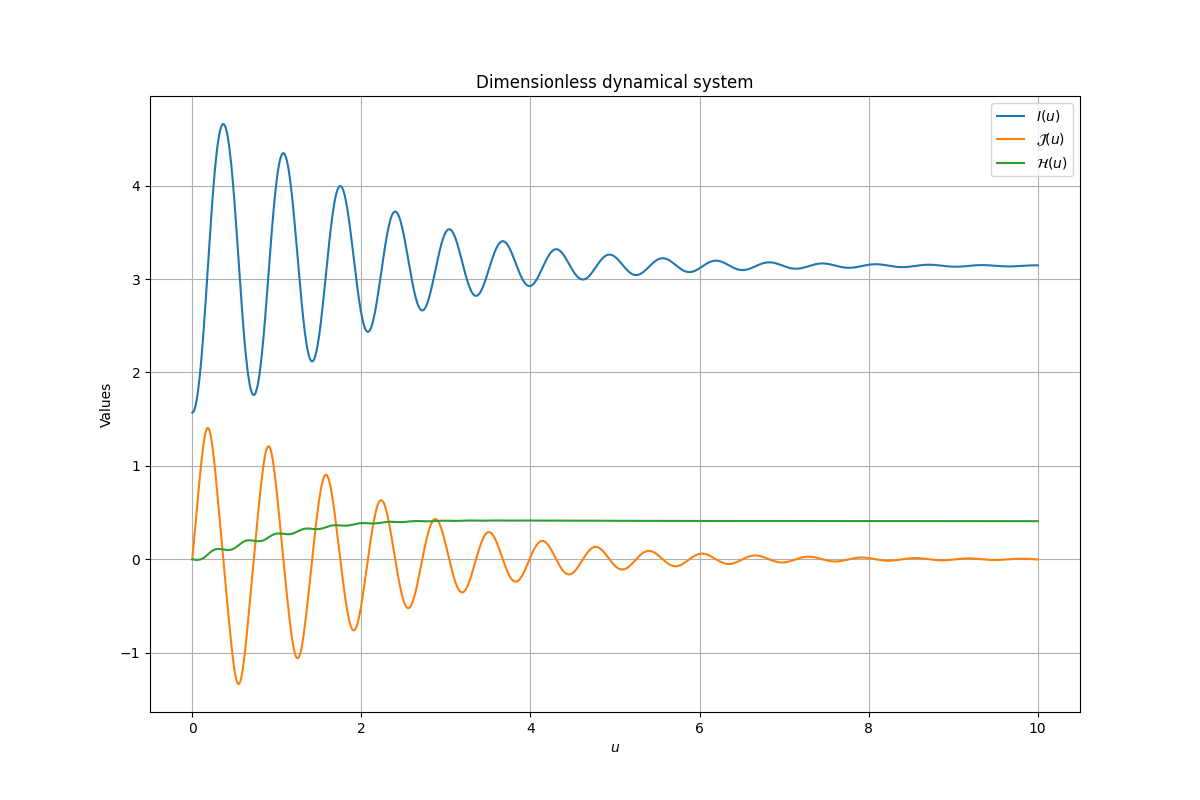
\includegraphics[width=0.72\textwidth]{d3v05alpha01.png}
\caption{The autonomous system with initial conditions: $\mathcal{J}=0,\,I = \frac{\pi}{2}\Rightarrow V(0) = V_1 v_0,\,\mathcal{H}=0$}
\label{fig:anexample}
\end{figure}

One can analytically derive that the critical points correspond to EAdS fixed points
\begin{equation}
  \mathcal{J}_\star =0 \sp I_\star = (2n+1)\pi \sp \mathcal{H}_\star = \pm \sqrt{\frac{2}{d(d-1)}\left(1-v_0\right)}\,.
\end{equation}
Let's look at the linear stability. Denoting $\delta X = (\delta I, \delta \mathcal{J}, \delta \mathcal{H})$ One finds the following system
\begin{equation}
  \frac{d\delta X}{d\eta} = \begin{pmatrix}
    0 && \frac{1}{\alpha} && 0 \\
    -\frac{1}{\alpha} && -d\mathcal{H}_{\star} && 0 \\
    0 && 0 && -2\mathcal{H}_\star 
  \end{pmatrix} \delta X \,,
\end{equation}
We first observe that $\lambda = -2\mathcal{H}_\star$ is an eigenvalue. First, requiring stability imposes the sign of $\mathcal{H}_\star>0$. We thus focus in such case. The remaining two eigenvalues solve a second order equation
\begin{equation}
  \lambda^2+d \mathcal{H}_ \star\lambda + \frac{1}{\alpha^2} = 0\,.
\end{equation}
We can observe that the system is always stable. The product of the eigenvalues is positive and the sum is negative which imposes that both eigenvalues have real negative part. Nevertheless, the phase portrait is affected by the value of the parameters. If 
\begin{equation}\label{eq:onsetspirals}
  \Delta < 0 \quad \text{i.e} \quad \frac{d}{(d-1)}(1-v_0)< \frac{2}{\alpha^2}\,,
\end{equation}
the orbits will be spiraling trajectories around the fixed point before reaching it. Otherwise, the orbits will directly flow to the fixed point. We can check that by drawing the phase portrait. Note that the $\chi$ particle describes a motion similar to a dissipative pendulum whose friction/anti-friction coefficient is time-dependent. This is natural to project the phase portrait into the plane $(I,\mathcal{J}) \sim (\chi, \Pi_{\chi})$. We display the phase portrait in the two distinct regimes.
\begin{figure}[h!]
\centering
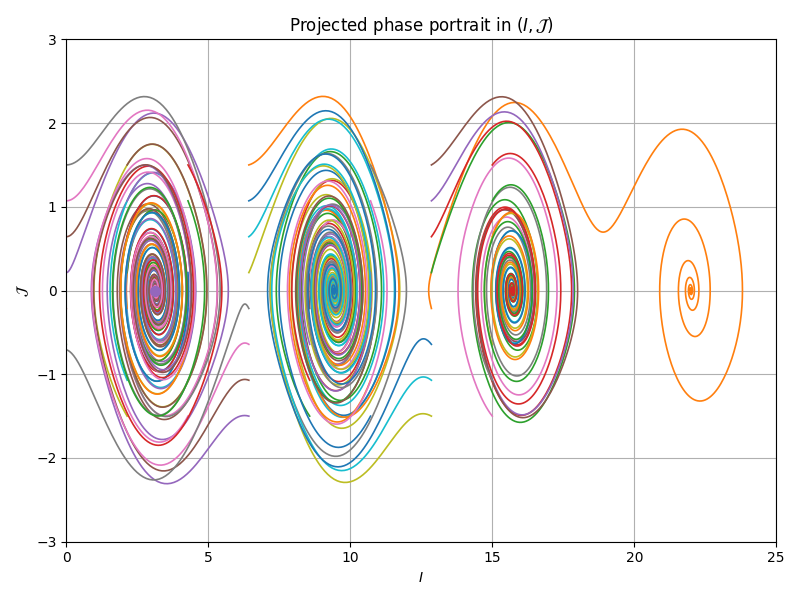
\includegraphics[width=0.72\textwidth]{projectedphaseportraitv05d3alpha02.png}
\caption{Phase portrait with parameter $v_0=0.5,\,\alpha = 0.2,\,d=3$ and initial conditions $\mathcal{H}(0)=0$. $\sim65$ orbits are displayed.}
\label{fig:phaseportrait1}
\end{figure}
As expected, in such regime, the motion of the $\chi$ particle is described by circular orbits in the phase portrait. This phase portrait is similar to the one we know for a pendulum. Nevertheless, it should be noted that it presents strking differences. Look at the orange curve to the right. It starts at a value of $I$ in $[3\pi,5\pi]$ but it ends in the critical point $\mathcal{I}_\star =7\pi$. This hints toward the fact that the system is dominated by friction than anti-friction. If it was not the case, trajectories could flow away to infinity.\\

\textbf{Conjecture:} All the trajectories end at a critical point.

This can be numerically inferred including more orbits at it is displayed in the following phase portrait.
\begin{figure}[h!]
\centering
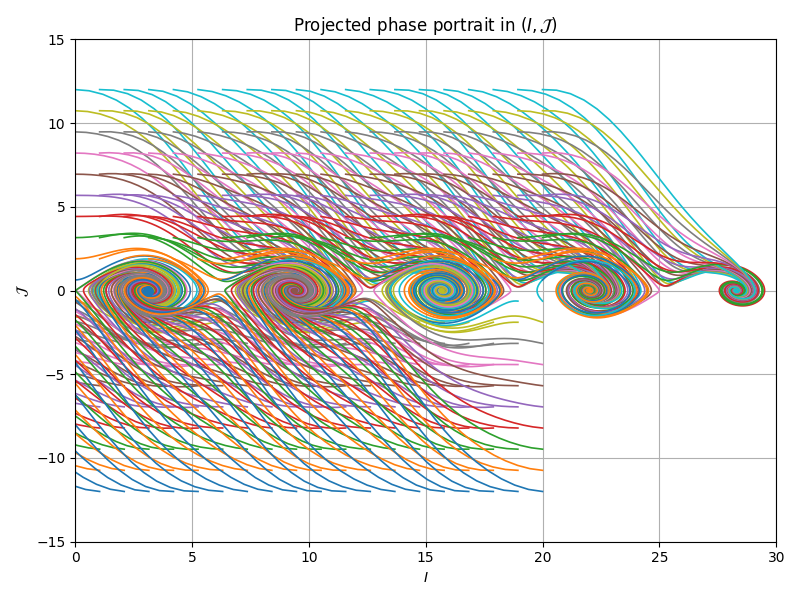
\includegraphics[width=0.72\textwidth]{phaseportraitv05alpha02d3.png}
\caption{Phase portrait with parameter $v_0=0.5,\,\alpha = 0.2,\,d=3$ and initial conditions $\mathcal{H}(0)=0$. $\sim400$ orbits are displayed.}
\label{fig:phaseportrait2}
\end{figure}

The second regime for which orbits are not circular show a rather different phase portrait.
\begin{figure}[h!]
\centering
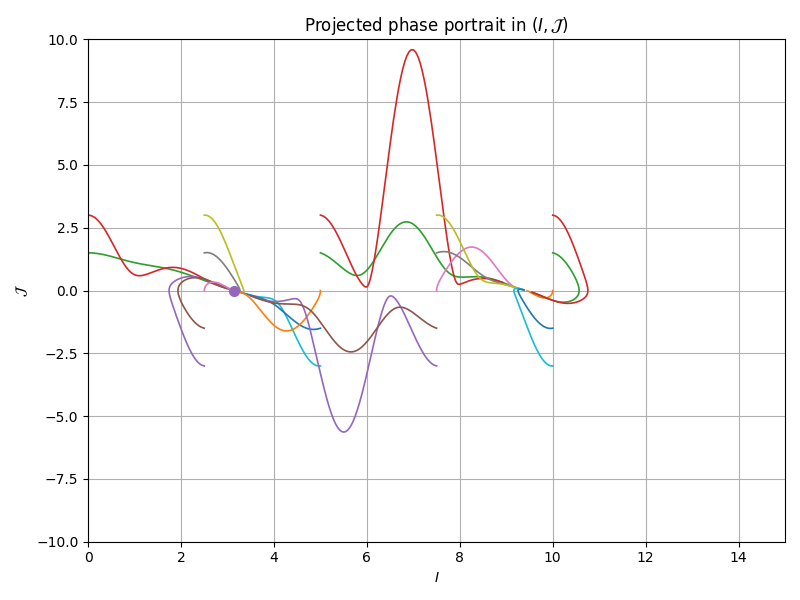
\includegraphics[width=0.72\textwidth]{phaseportraitv05alpha2d3.png}
\caption{Phase portrait with parameter $v_0=0.5,\,\alpha = 2,\,d=3$ and initial conditions $\mathcal{H}(0)=0$. $\sim30$ orbits are displayed.}
\label{fig:phaseportrait3}
\end{figure}

\subsection{Holographic properties of the solutions.}
In this paragraph, we describe the holographic properties of the domain-wall solutions which
asymptote to the EAdS fixed point. Near the AdS fixed point,
\begin{equation}
  V(\chi)\to V_0-V_1<0\,.
\end{equation}
The spacetime asymptotes to an AdS geometry with length $L_{\rm AdS}$. In terms of the
dimensionless variable $\mathcal H=H/M$, one has
\begin{equation}
  M L_{\rm AdS}
  =
  \frac{1}{|\mathcal H_\star|}
  =
  \sqrt{\frac{d(d-1)}{2(1-v_0)}}\,.
\end{equation}
Equivalently,
\begin{equation}
  L_{\rm AdS}
  =
  \sqrt{
  \frac{d(d-1)}
  {2\kappa V_1(1-v_0)}
  }\,.
\end{equation}
Expanding around the fixed point
$\chi_\star=(2n+1)\pi f_\chi$, and writing
$\delta\chi=\chi-\chi_\star$, one obtains
\begin{equation}
  V(\chi)
  =
  V_0-V_1
  +
  \frac{V_1}{2f_\chi^2}(\delta\chi)^2
  +
  \mathcal O((\delta\chi)^4)\,.
\end{equation}
Because the Euclidean axion has the wrong-sign kinetic term, the mass parameter entering the
standard holographic scalar equation is
\begin{equation}
  m_{\rm holo}^2
  =
  -m_{\rm axion}^2
  =
  -\frac{V_1}{f_\chi^2}
  =
  -\frac{M^2}{\alpha^2}\,.
\end{equation}
Thus
\begin{equation}
  m_{\rm holo}^2L_{\rm AdS}^2
  =
  -
  \frac{d(d-1)}{2\alpha^2(1-v_0)}
  <0\,.
\end{equation}
In the standard quantization, provided the BF bound is satisfied, this corresponds to a relevant
deformation with $\Delta_+<d$. The BF bound requires
\begin{equation}
  m_{\rm holo}^2L_{\rm AdS}^2\geq -\frac{d^2}{4}.
\end{equation}
For sufficiently small $\alpha^2(1-v_0)$, the BF bound is violated. Interestingly, this bound has also been infered previously at the onset for which the orbits are spiraling trajectories~\eqref{eq:onsetspirals}. Therefore the onset of spiralling in the linearized phase portrait coincides with the violation of the BF bound of the asymptotic EAdS fixed point. If the fixed point is to define a stable holographic UV/IR endpoint, the spiralling regime should be excluded. In particular, none of the solutions satisfying the BF bound can pass through the minimum of the potential without vanishing velocity. Consider now the case where the BF bound is satisfied. Let us show that the charge of the axion blows up at the AdS boundary. To see why, first observe that the scale factor behaves (in units of AdS length) as $a(\tau)\sim e^{\tau}$. We then expand the axion field as
\begin{equation}
  \chi(\tau) = \chi_{(-)} e^{-\Delta_- \tau} + \chi_{(1)}e^{-\left(\Delta_- + 1\right)\tau} + \cdots + \chi_{(+)} e^{-\Delta_+ \tau} + \cdots\,,
\end{equation}
where in Neumann quantization shceme, $\chi_-$ corresponds to the VEV of the dual operator and $\chi_{(+)}$ corresponds to the source. We first remark that the finiteness of the charge $Q(\tau)\sim a^d \partial_\tau \chi$ of the boundary imposes the vev to vanish. Then, since the deformation is relevant, we have $\Delta_+ \leq d$ (where in the equal case we are eventually back to the non-running solutions). We conclude that the charge of the axion blows up at the AdS boundary for running solutions. The solutions describe infinite flux at the AdS boundary. We thus conclude with a very general theorem\\
\textbf{Theorem}: For asymptotically EAdS running solutions satisfying the BF bound for which both modes are normalizable $d>\Delta_+>0,\Delta_->0$, finite boundary flux forces both asymptotic coefficients to vanish. Hence any non-trivial running solution carries infinite axionic flux at the EAdS boundary.
(\textit{In our specific setup, the holographic mass is always negative and thus the deformation always satisfies $\Delta_+<d$.})
\paragraph{Finite action and counter-terms}
We consider the case where the BF bound is satisfied. We would like to find a way numerically to regulate the action and compute it numerically as a function of the UV parameters. It actually highly depends on the the dimension of the axion dual operator $\Delta_+$ and thus on the dimension and the parameters $\alpha,v_0$. Consider the case where the boundary dimension is $d=3$ and $\Delta_+=2$. In such a case, the relevant counter-terms to render the action finite are
\begin{equation}
  \begin{aligned}
S_{\rm ct}
&=
\frac{1}{\kappa}
\int_{\partial M} d^3x\sqrt{\gamma}
\left(
2H_{\rm AdS}
+
\frac{1}{2H_{\rm AdS}}R[\gamma]
- 2 H_{\rm AdS}(\delta\chi)^2
\right)\\
&=
\frac{{\rm Vol}(S^3)}{\kappa}
\left(
2H_{\rm AdS}a_R^3+\frac{3a_R}{H_{\rm AdS}} - 2 H_{\rm AdS}a_R^3(\delta\chi)^2(\tau_R)
\right)\,.
\end{aligned}
\end{equation}

\end{document}

